\documentclass[12pt, a4paper, oneside, UTF8]{ctexart}
\usepackage{amsmath, amsthm, amssymb, bm, color, framed, graphicx, hyperref, mathrsfs}
\usepackage{geometry}
\geometry{left = 2.5 cm, right = 2.5 cm, top = 2.5 cm, bottom = 2.5 cm}

\title{\textbf{作业6}\\{\small (数值算法与案例分析)}}
\author{李维杰}
\date{\today}
\linespread{1.5}
\definecolor{shadecolor}{RGB}{241, 241, 255}
\newcounter{problemname}
\newenvironment{problem}{\begin{shaded}\stepcounter{problemname}\par\noindent\textbf{题目\arabic{problemname}. }}{\end{shaded}\par}
\newenvironment{solution}{\par\noindent\textbf{解答. }}{\par}
\newenvironment{note}{\par\noindent\textbf{注记. }}{\par}

\begin{document}

\maketitle

\begin{problem}
    设有瘦高上双对角矩阵$A\in{\mathbb{R}^{{m}\times{n}}}$(即$a_{i,j}\neq0$当且仅当$i-j\in\{0,-1\}$).设计一个基于Givens Rotations的算法解决岭回归问题
    $$\min{\left\lVert{Ax-b}\right\rVert}_{\mathsf{2}}^{2}+\lambda{\left\lVert{x}\right\rVert}_{2}^{2},$$
    其中$\lambda$是一个给定的正数.
\end{problem}

\begin{solution}
    问题等价于标准最小二乘问题
    \begin{align*}
        \min_{Cx=d}{\left\lVert{\left[
            \begin{array}{cc}	
                A \\
                \sqrt{\lambda}I
            \end{array}
        \right]x-\left[
            \begin{array}{cc}	
                b \\
                0
            \end{array}
        \right]}\right\rVert}_{\mathsf{2}}.
    \end{align*}
    此问题的法方程为
    \begin{align*}
        \left[
            \begin{array}{cc}	
                A \\
                \sqrt{\lambda}I
            \end{array}
        \right]^*
        \left[
            \begin{array}{cc}	
                A \\
                \sqrt{\lambda}I
            \end{array}
        \right]x
        =
        \left[
            \begin{array}{cc}	
                A \\
                \sqrt{\lambda}I
            \end{array}
        \right]^*
        \left[
            \begin{array}{cc}	
                b \\
                0
            \end{array}
        \right].
    \end{align*}
    即
    \begin{align*}
        (A^*A+\lambda{I})x=A^*b.
    \end{align*}
    其中,$A^*A+\lambda{I}$是一个三对角阵,故可以使用$n$次Givens Rotations,将$A^*A+\lambda{I}$变换为上双对角阵,也即上三角阵$R$.
    同时,将这$n$次Givens Rotations作用于$A^*b$得到向量$c$,最后解线性方程组$Rx=c$即可.
\end{solution}

\begin{problem}
    设计一个基于Gaussian elimination消去约束系统的算法解决带约束的最小二乘问题
    $$\min\limits_{Cx=d}{\left\lVert{Ax-b}\right\rVert}_{\mathsf{2}}.$$
\end{problem}

\begin{solution}
    对$Cx=d$做Gaussian elimination,得
    \begin{align*}
        \left[
            \begin{array}{cc}	
                R & C_2
            \end{array}
        \right]
        \left[
            \begin{array}{cc}	
                x_1 \\
                x_2
            \end{array}
        \right]
        = d'.
    \end{align*}
    其中,$\left[
        \begin{array}{cc}	
            R & C_2
        \end{array}
    \right]$是一个梯形矩阵.于是解得
    $$x_1 = R^{-1}(d'-C_2x_2).$$
    按$\left[
        \begin{array}{cc}	
            x_1 & x_2
        \end{array}
    \right]$的规模大小对$A$分块为$A=\left[
        \begin{array}{cc}	
            A_1 & A_2
        \end{array}
    \right]$,则
    \begin{align*}
        \min\limits_{Cx=d}{\left\lVert{Ax-b}\right\rVert}_{2}&=\min{\left\lVert{A_1x_1+A_2x_2-b}\right\rVert}_{2}\\
        &=\min{\left\lVert{(A_2-A_1R^{-1}C_2)x_2-(b-A_1R^{-1}d')}\right\rVert}_{2}.
    \end{align*}
\end{solution}

\begin{problem}
    最小二乘问题$\min{\left\lVert{Ax-b}\right\rVert}_{2}$等价于Hermite不定增广线性系统
    \begin{align*}
        \left[
            \begin{array}{cc}	
                I & A \\
                A^* & 0
            \end{array}
        \right]
        \left[
            \begin{array}{cc}	
                r \\
                x
            \end{array}
        \right]
        =
        \left[
            \begin{array}{cc}	
                b \\
                0
            \end{array}
        \right],
    \end{align*}
    对于带约束的最小二乘问题$\min\limits_{Cx=d}{\left\lVert{Ax-b}\right\rVert}_{2}$,同样存在类似的增广线性系统,请找出它.
\end{problem}

\begin{solution}
    \textbf{算法1.} $\min\limits_{Cx=d}{\left\lVert{Ax-b}\right\rVert}_{2}$对应的增广线性系统为
    \begin{align*}
        \left[
            \begin{array}{cc}	
                A^*A & C^* \\
                C & 0
            \end{array}
        \right]
        \left[
            \begin{array}{cc}	
                \hat{x} \\
                z
            \end{array}
        \right]
        =
        \left[
            \begin{array}{cc}	
                A^*b \\
                d
            \end{array}
        \right].
    \end{align*}
    事实上,假设存在其它满足$Cx=d$的$x$,且有$x\neq\hat{x}$,下面证明
    $${\left\lVert{Ax-b}\right\rVert}_{2}\geqslant{\left\lVert{A\hat{x}-b}\right\rVert}_{2}$$即可.\\
    由于$A^*A\hat{x}+C^*z=A^*b$,可知$A^*(A\hat{x}-b)=-C^*z$,故
    \begin{align*}
        2(x-\hat{x})^*A^*(A\hat{x}-b)&=-2(x-\hat{x})^*C^*z\\
        &=-2[C(x-\hat{x})]^*z\\
        &=0.
    \end{align*}
    于是
    \begin{align*}
        {\left\lVert{Ax-b}\right\rVert}_{2}^{2}&={\left\lVert{A(x-\hat{x})+A\hat{x}-b}\right\rVert}_{2}^{2}\\
        &={\left\lVert{A(x-\hat{x})}\right\rVert}_{2}^{2}+{\left\lVert{A\hat{x}-b}\right\rVert}_{2}^{2}+2(x-\hat{x})^*A^*(A\hat{x}-b)\\
        &={\left\lVert{A(x-\hat{x})}\right\rVert}_{2}^{2}+{\left\lVert{A\hat{x}-b}\right\rVert}_{2}^{2}\\
        &\geqslant {\left\lVert{A\hat{x}-b}\right\rVert}_{2}^{2}
    \end{align*}
    当且仅当$x=\hat{x}$时取等.\\
    \textbf{算法2.} 设Lagrange函数
    $$L(x,\lambda) = \frac{1}{2}({\left\lVert{Ax-b}\right\rVert}_{2}^{2}+\lambda{\left\lVert{Cx-d}\right\rVert}_{2}^{2}),$$
    令
    \begin{align*}
        \left\{
            \begin{array}{ll}
                \frac{\partial{L}}{\partial{x}} = A^*(A\hat{x}-b)+\lambda{C^*}(Cx-d) = 0 \\
                C\hat{x}-d = 0
            \end{array}
        \right.,
    \end{align*}
    则$\min\limits_{Cx=d}{\left\lVert{Ax-b}\right\rVert}_{2}$对应的增广线性系统为
    \begin{align*}
        \left[
            \begin{array}{ccc}	
                I & A \\
                A^* & 0 \\
                0 & C
            \end{array}
        \right]
        \left[
            \begin{array}{ccc}	
                b-A\hat{x} \\
                \hat{x}
            \end{array}
        \right]
        =
        \left[
            \begin{array}{ccc}	
                b \\
                0 \\
                d
            \end{array}
        \right].
    \end{align*}
\end{solution}
\newpage
\begin{problem}
    分别使用CGS/CGS2/MGS/MGS2算法进行Arnoldi过程并可视化正交性损失.
    使用的样例可以是随机生成的$1000\times1000$矩阵和$30$维的Krylov subspace.
\end{problem}

\begin{solution}
    (代码见Problem4.m)
    \begin{figure}[htbp] % 创建一个图形环境
        \centering % 图片居中
        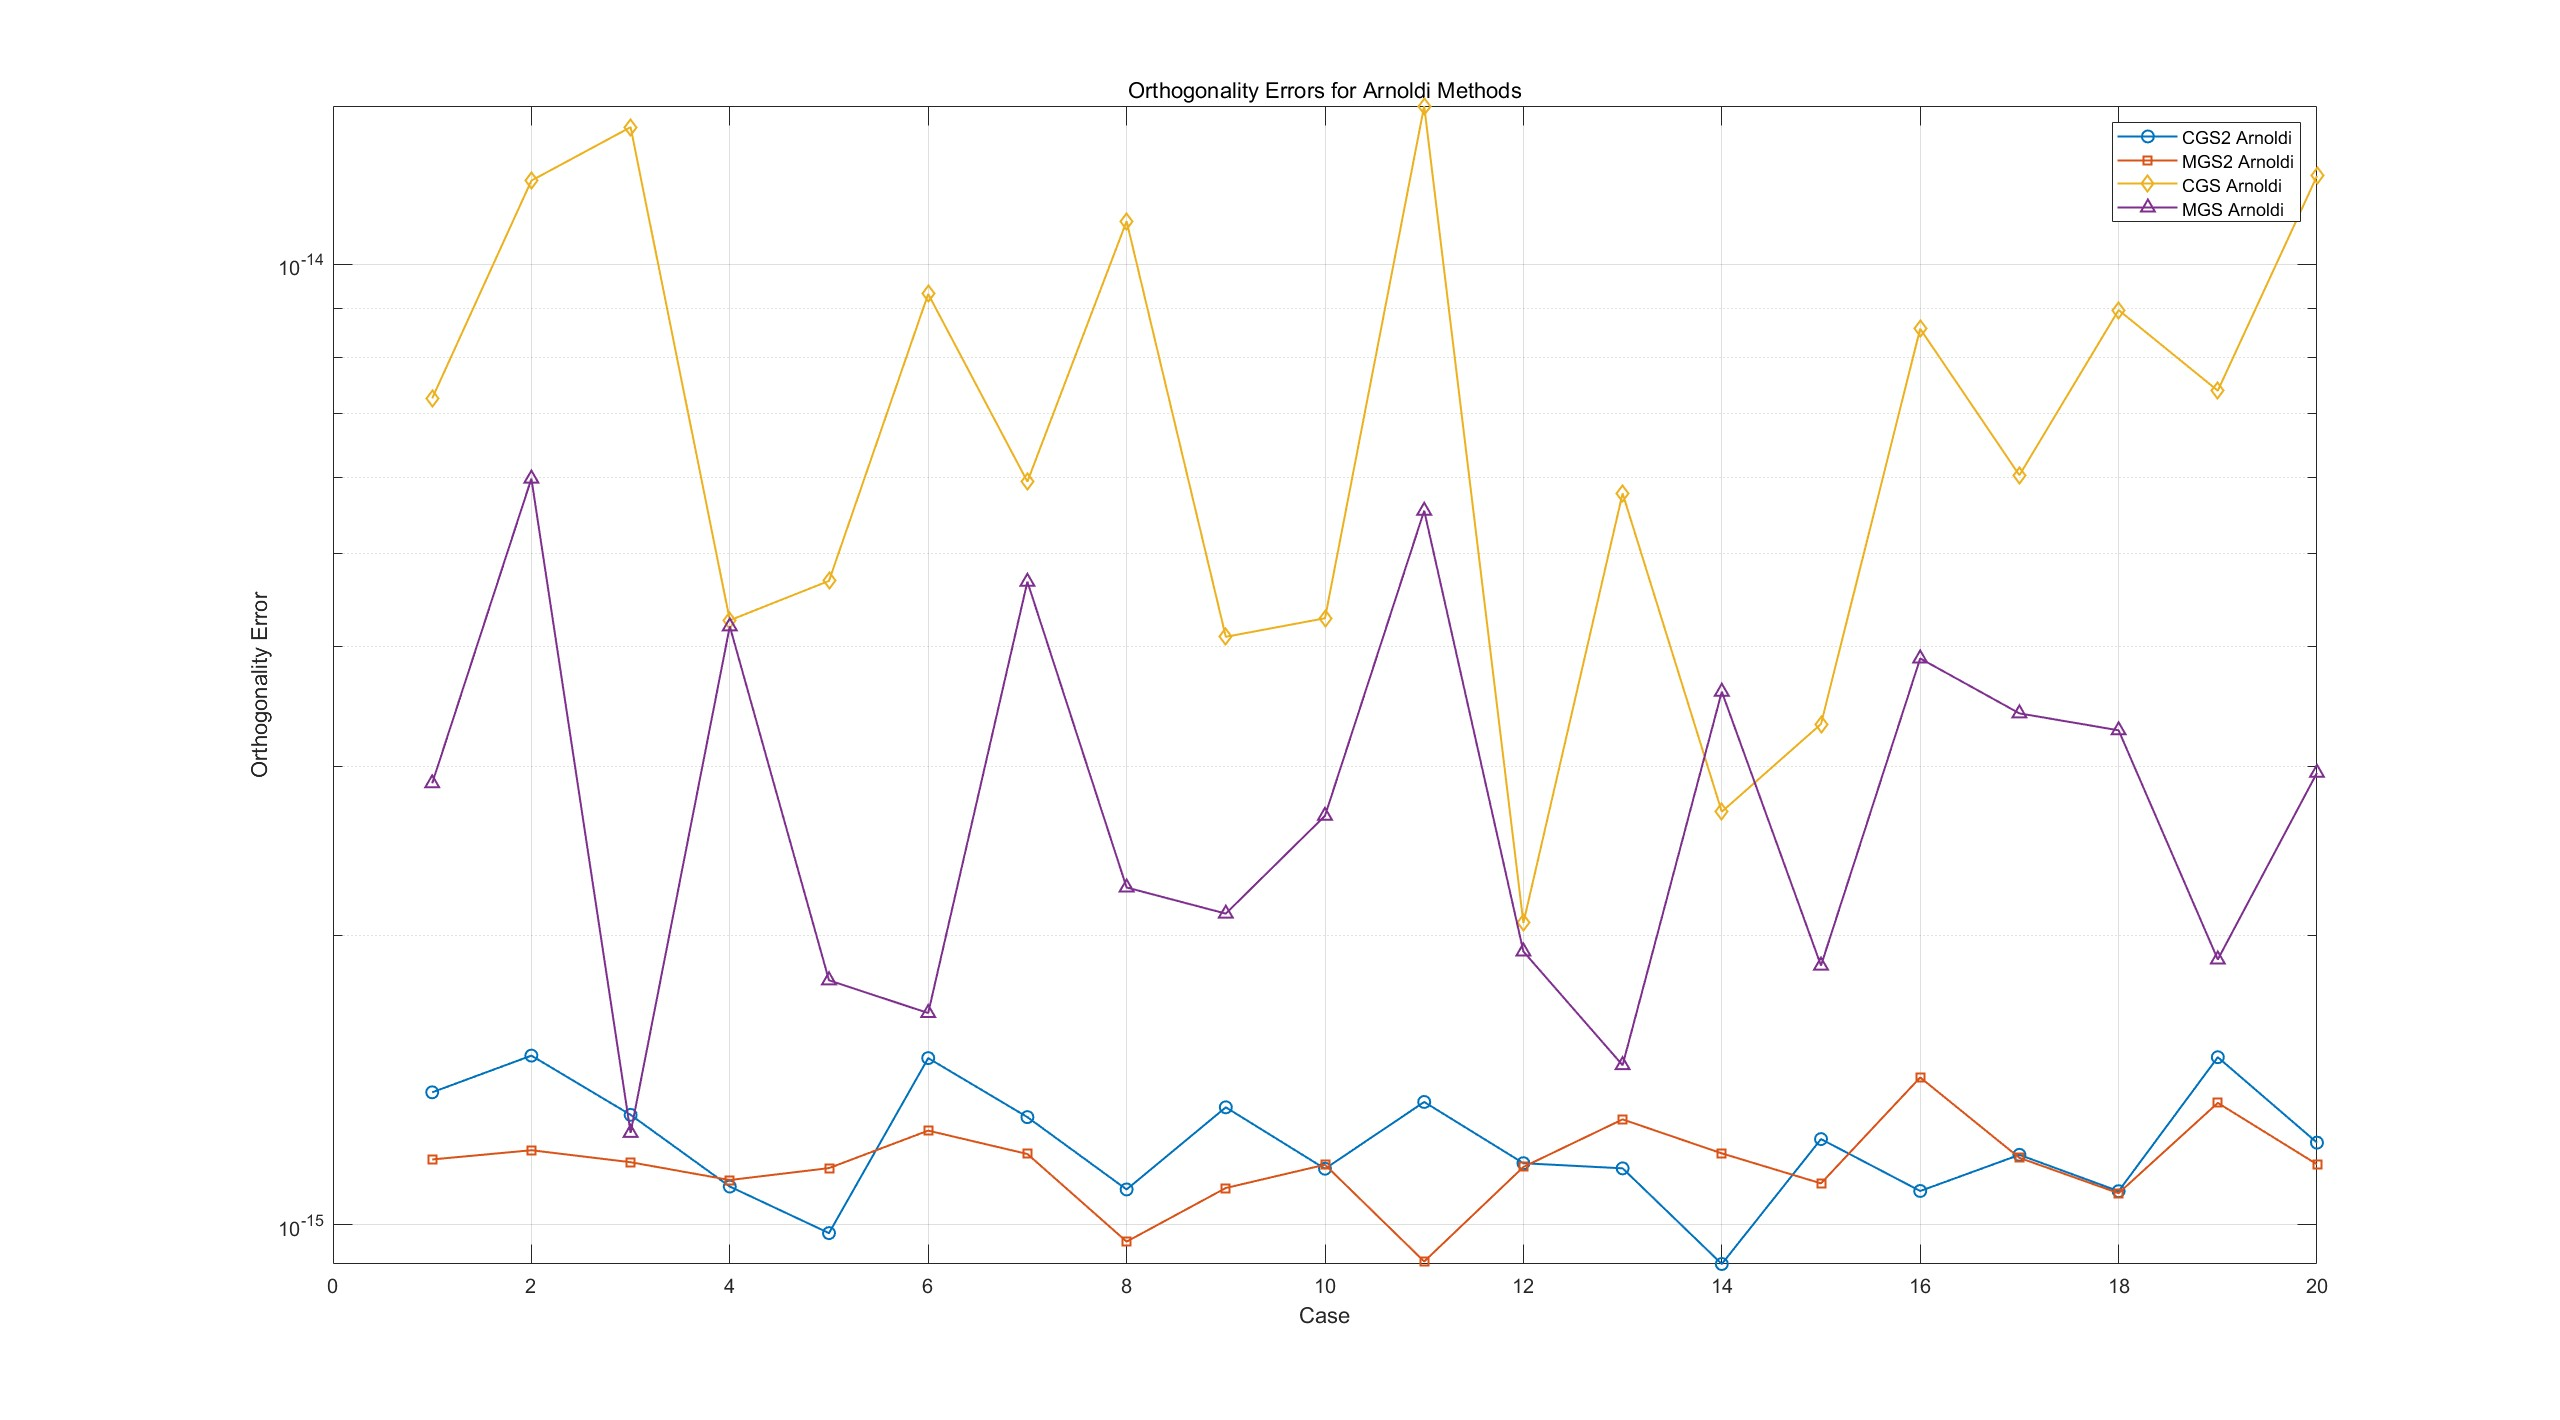
\includegraphics[scale=0.17]{Problem4.jpg} % 插入图片,设置宽度为页面宽度的70%
        \caption{四种算法在20种随机样例下的正交性损失${\left\lVert{Q^*Q-I_n}\right\rVert}_{\mathsf{F}}$} % 图片的说明文字
    \end{figure}
\end{solution}

\begin{problem}
    假设矩阵的秩已经给定,编写一个程序来解决亏秩最小二乘问题.
\end{problem}

\begin{solution}
    通过列选主元的QR分解求得亏秩条件下的最小二乘解为$\hat{x}$,
    并设满秩条件下的最小二乘解为$\tilde{x}=(A^*A)^{-1}A^*b$.
    对于随机生成的亏秩最小二乘问题$(A,b)$,两种解与观测值之间的差异度为
    $${\left\lVert{A\hat{x}-b}\right\rVert}_{2}={\left\lVert{A\tilde{x}-b}\right\rVert}_{2}=0.2723.$$
    且$\hat{x}_i\neq{0}$当且仅当$col(A)_i$是列空间$C(A)$的一个基.(代码见Problem5.m)
\end{solution}
\end{document}